\documentclass[uplatex,dvipdfmx,a4paper,11pt]{jsarticle}

\usepackage{docmute}


% 数式
\usepackage{amsmath,amsthm,amssymb}
\usepackage{bm}
% 画像
\usepackage{graphicx}

\usepackage{multirow}
\usepackage{wrapfig}
\usepackage{ascmac}
\usepackage{xcolor}


\usepackage{makeidx}
\makeindex

\graphicspath{{../../_Figures//}{../../_Figures/Rheology/}}

\usepackage{qrcode}
\setlength\lineskiplimit{0pt}
\setlength\normallineskiplimit{0pt}

\usepackage{qexam}

\usepackage{titlesec}
\titleformat*{\section}{\Large\bfseries}
\titleformat*{\subsection}{\large\bfseries}
\titleformat*{\subsubsection}{\normalsize\bfseries}
\titleformat*{\paragraph}{\normalsize\bfseries}

% ページ設定
% \pagestyle{empty}
% 高さの設定
\setlength{\textheight}{\paperheight}   % ひとまず紙面を本文領域に
\setlength{\topmargin}{-5.4truemm}      % 上の余白を20mm(=1inch-5.4mm)に
\addtolength{\topmargin}{-\headheight}  % 
\addtolength{\topmargin}{-\headsep}     % ヘッダの分だけ本文領域を移動させる
\addtolength{\textheight}{-40truemm}    % 下の余白も20mmに%% 幅の設定
\setlength{\textwidth}{\paperwidth}     % ひとまず紙面を本文領域に
\setlength{\oddsidemargin}{-5.4truemm}  % 左の余白を20mm(=1inch-5.4mm)に
\setlength{\evensidemargin}{-5.4truemm} % 
\addtolength{\textwidth}{-40truemm}     % 右の余白も20mmに
% 図と本文との間
%\abovecaptionskip=-5pt
%\belowcaptionskip=-5pt
%
% 全体の行間調整
% \renewcommand{\baselinestretch}{1.0} 
% 図と表
%\renewcommand{\figurename}{Fig.}
%\renewcommand{\tablename}{Tab.}
%

% \makeatletter 
% \def\section{\@startsection {section}{1}{\z@}{1.5 ex plus 2ex minus -.2ex}{0.5 ex plus .2ex}{\large\bf}}
% \def\subsection{\@startsection{subsection}{2}{\z@}{0.2\Cvs \@plus.5\Cdp \@minus.2\Cdp}{0.1\Cvs \@plus.3\Cdp}{\reset@font\normalsize\bfseries}}
% \makeatother 

\usepackage[dvipdfmx,%
 bookmarks=true,%
 bookmarksnumbered=true,%
 colorlinks=false,%
 setpagesize=false,%
 pdftitle={数式に頼らない直感的理解による材料設計のためのレオロジー⼊⾨},%
 pdfauthor={佐々木裕},%
 pdfsubject={},%
 pdfkeywords={レオロジー; 材料設計; }]{hyperref}
\usepackage{pxjahyper}

\usepackage{plext}

\usepackage{niceframe} 
\usepackage{framed}
\newenvironment{longartdeco}{%
  \def\FrameCommand{\fboxsep=\FrameSep \artdecoframe}%
  \MakeFramed {\FrameRestore}}%
 {\endMakeFramed}
 
\usepackage{siunitx}

\newcommand{\rmd}{\mathrm{d}}

\usepackage[inline]{showlabels}

\begin{document}

\section*{この章の内容}

ここでは、レオロジーという「考え方」についての説明から始めていきます。
レオロジーを学ぶことで会社の仕事に活かせるような考え方を身に付けていただきたいと思います。

以下に、この章で議論する内容について簡単にまとめました。

\begin{boxnote}
	\large
	\begin{itemize}
		\item レオロジーとは?\\はじめに、「レオロジー」という言葉について、概観しましょう。
		\begin{itemize}
			\item レオロジーの歴史的背景を振り返り、その流れを確認します。
			\item 具体的なレオロジーのやり方について説明します。
		\end{itemize} 
		\item 会社の仕事とレオロジー\\会社の仕事とレオロジーの関わりについて考えてみます。
		\begin{itemize}
			\item レオロジーが関わる分野が非常に広範囲に渡ることを確認します。
			\item 会社の仕事とレオロジーの関わりについて考えてみます。
			\item 特に商品を作り出すときの有効性について見てみます。
		\end{itemize} 
		\item 人の感覚とレオロジー\\人間の直感とレオロジーとの親和性が高いことについて考えてみます。
		\begin{itemize}
			\item レオロジーは、「おさわりの科学」とも言われています。
			\item 人間の五感が大事であることを再確認します。
			\item そして、人間の判断基準についても説明します。
		\end{itemize}
		\item レオロジーを理解するために\\有用なレオロジーですが、その理解は困難な場合も多く見受けられます。
		\begin{itemize}
			\item レオロジーの理解を妨げる要因について簡単にまとめます。
			\item おすすめの理解へのアプローチについて紹介します。
		\end{itemize} 
	\end{itemize}
\end{boxnote}

\section{レオロジーとは?}

まず、レオロジーという言葉のはじまりを確認し、どのような考え方であるのかを概観していきましょう。

\subsection{レオロジーの始まり}
1929年にアメリカにおいてレオロジー学会 The Society of Rheology (SOR) が設立されました。
このとき、中心となったのが、E.C. Bingham でした。
レオロジーという言葉は彼の造語であり、万物流転という意味を表すギリシア語の ``\textit{panta rhei}'' から引いた接頭語である ``Rheo-'' を学問の分野を表す ``-logy'' と組み合わせたものです。
そして、その対象を「物質の変形と流動\index{りゅうどう@流動}に関する科学」と定めたのでした。
\begin{figure}[htb]
	\begin{center}
		\begin{minipage}{0.5\textwidth}
			\large
			\begin{itembox}[l]{レオロジーの始まり}
				レオロジー (Rheology) とは、\\
			「物質の変形と流動に関する科学」
				\begin{itemize}
					\item \textit{panta rhei} (ギリシア語)
					\item ``everything flows''
					\item 万物流転
				\end{itemize}
			\end{itembox}
		\end{minipage}
		\begin{minipage}{0.4\textwidth}
			\begin{center}
				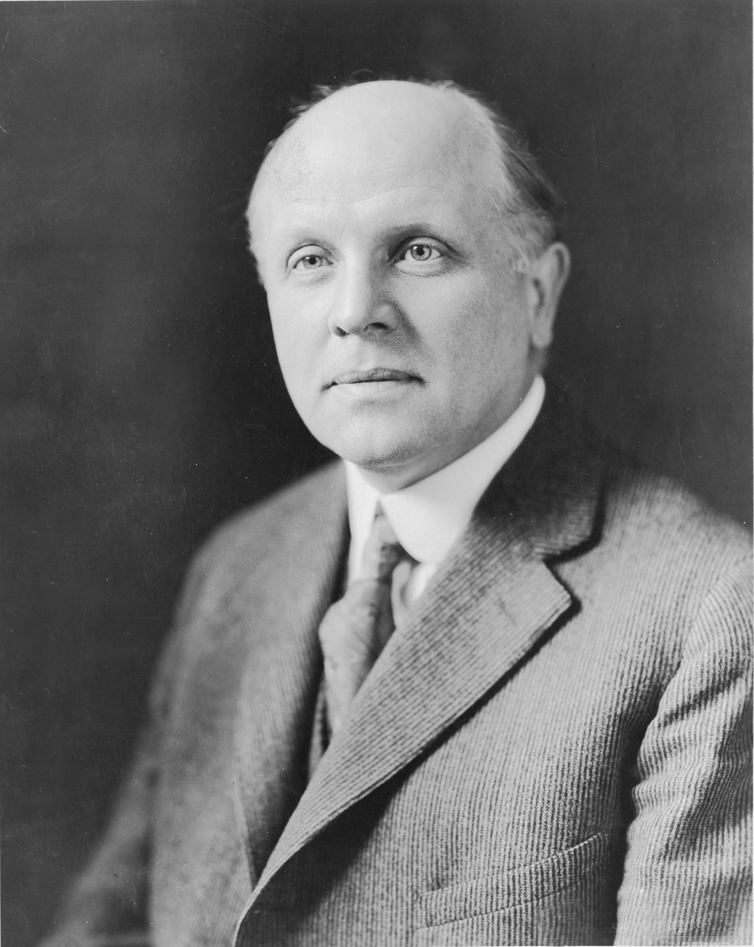
\includegraphics[width=0.6\textwidth]{Bingham.jpg}\\
				\large{\bf Eugene Cook Bingham}
			\end{center}
		\end{minipage}
	\end{center}
		\caption{レオロジーの創始者}
		\label{Bingham}
\end{figure}

日本では、それから約二十年後の 1951 年に第1回レオロジー討論会が開催されています。
学会としてレオロジー学会が設立されたのは、その二十年以上後の 1973 年になります。
ですから、学問と考えれば、それほど歴史が古いわけでもないことになります。
その後、現在に至るまでその発展は続いており、非常に多様な分野へと適応される範囲は広がってきています。

\subsection{レオロジーのやり方}

そもそも、物体の変形や流動\index{りゅうどう@流動}に関する物理学は、古くから弾性論\index{だんせいろん@弾性論}や流体論\index{りゅうたいろん@流体論}として存在していました。
弾性論は Hooke の法則\index{ふっくのほうそく@Hooke の法則}を基本にして弾性固体\index{こたい@固体}を、そして、流体論はNewton の法則\index{ニュートンの法則@Newton の法則}により粘性を持つ単純な流体を対象として、物体の挙動を明確にしていたのでした
\footnote{
	Hooke の法則、Newton の法則については、後ほどきちんと説明しますので、安心してください。
}。
\begin{figure}[htb]
    \begin{center}
        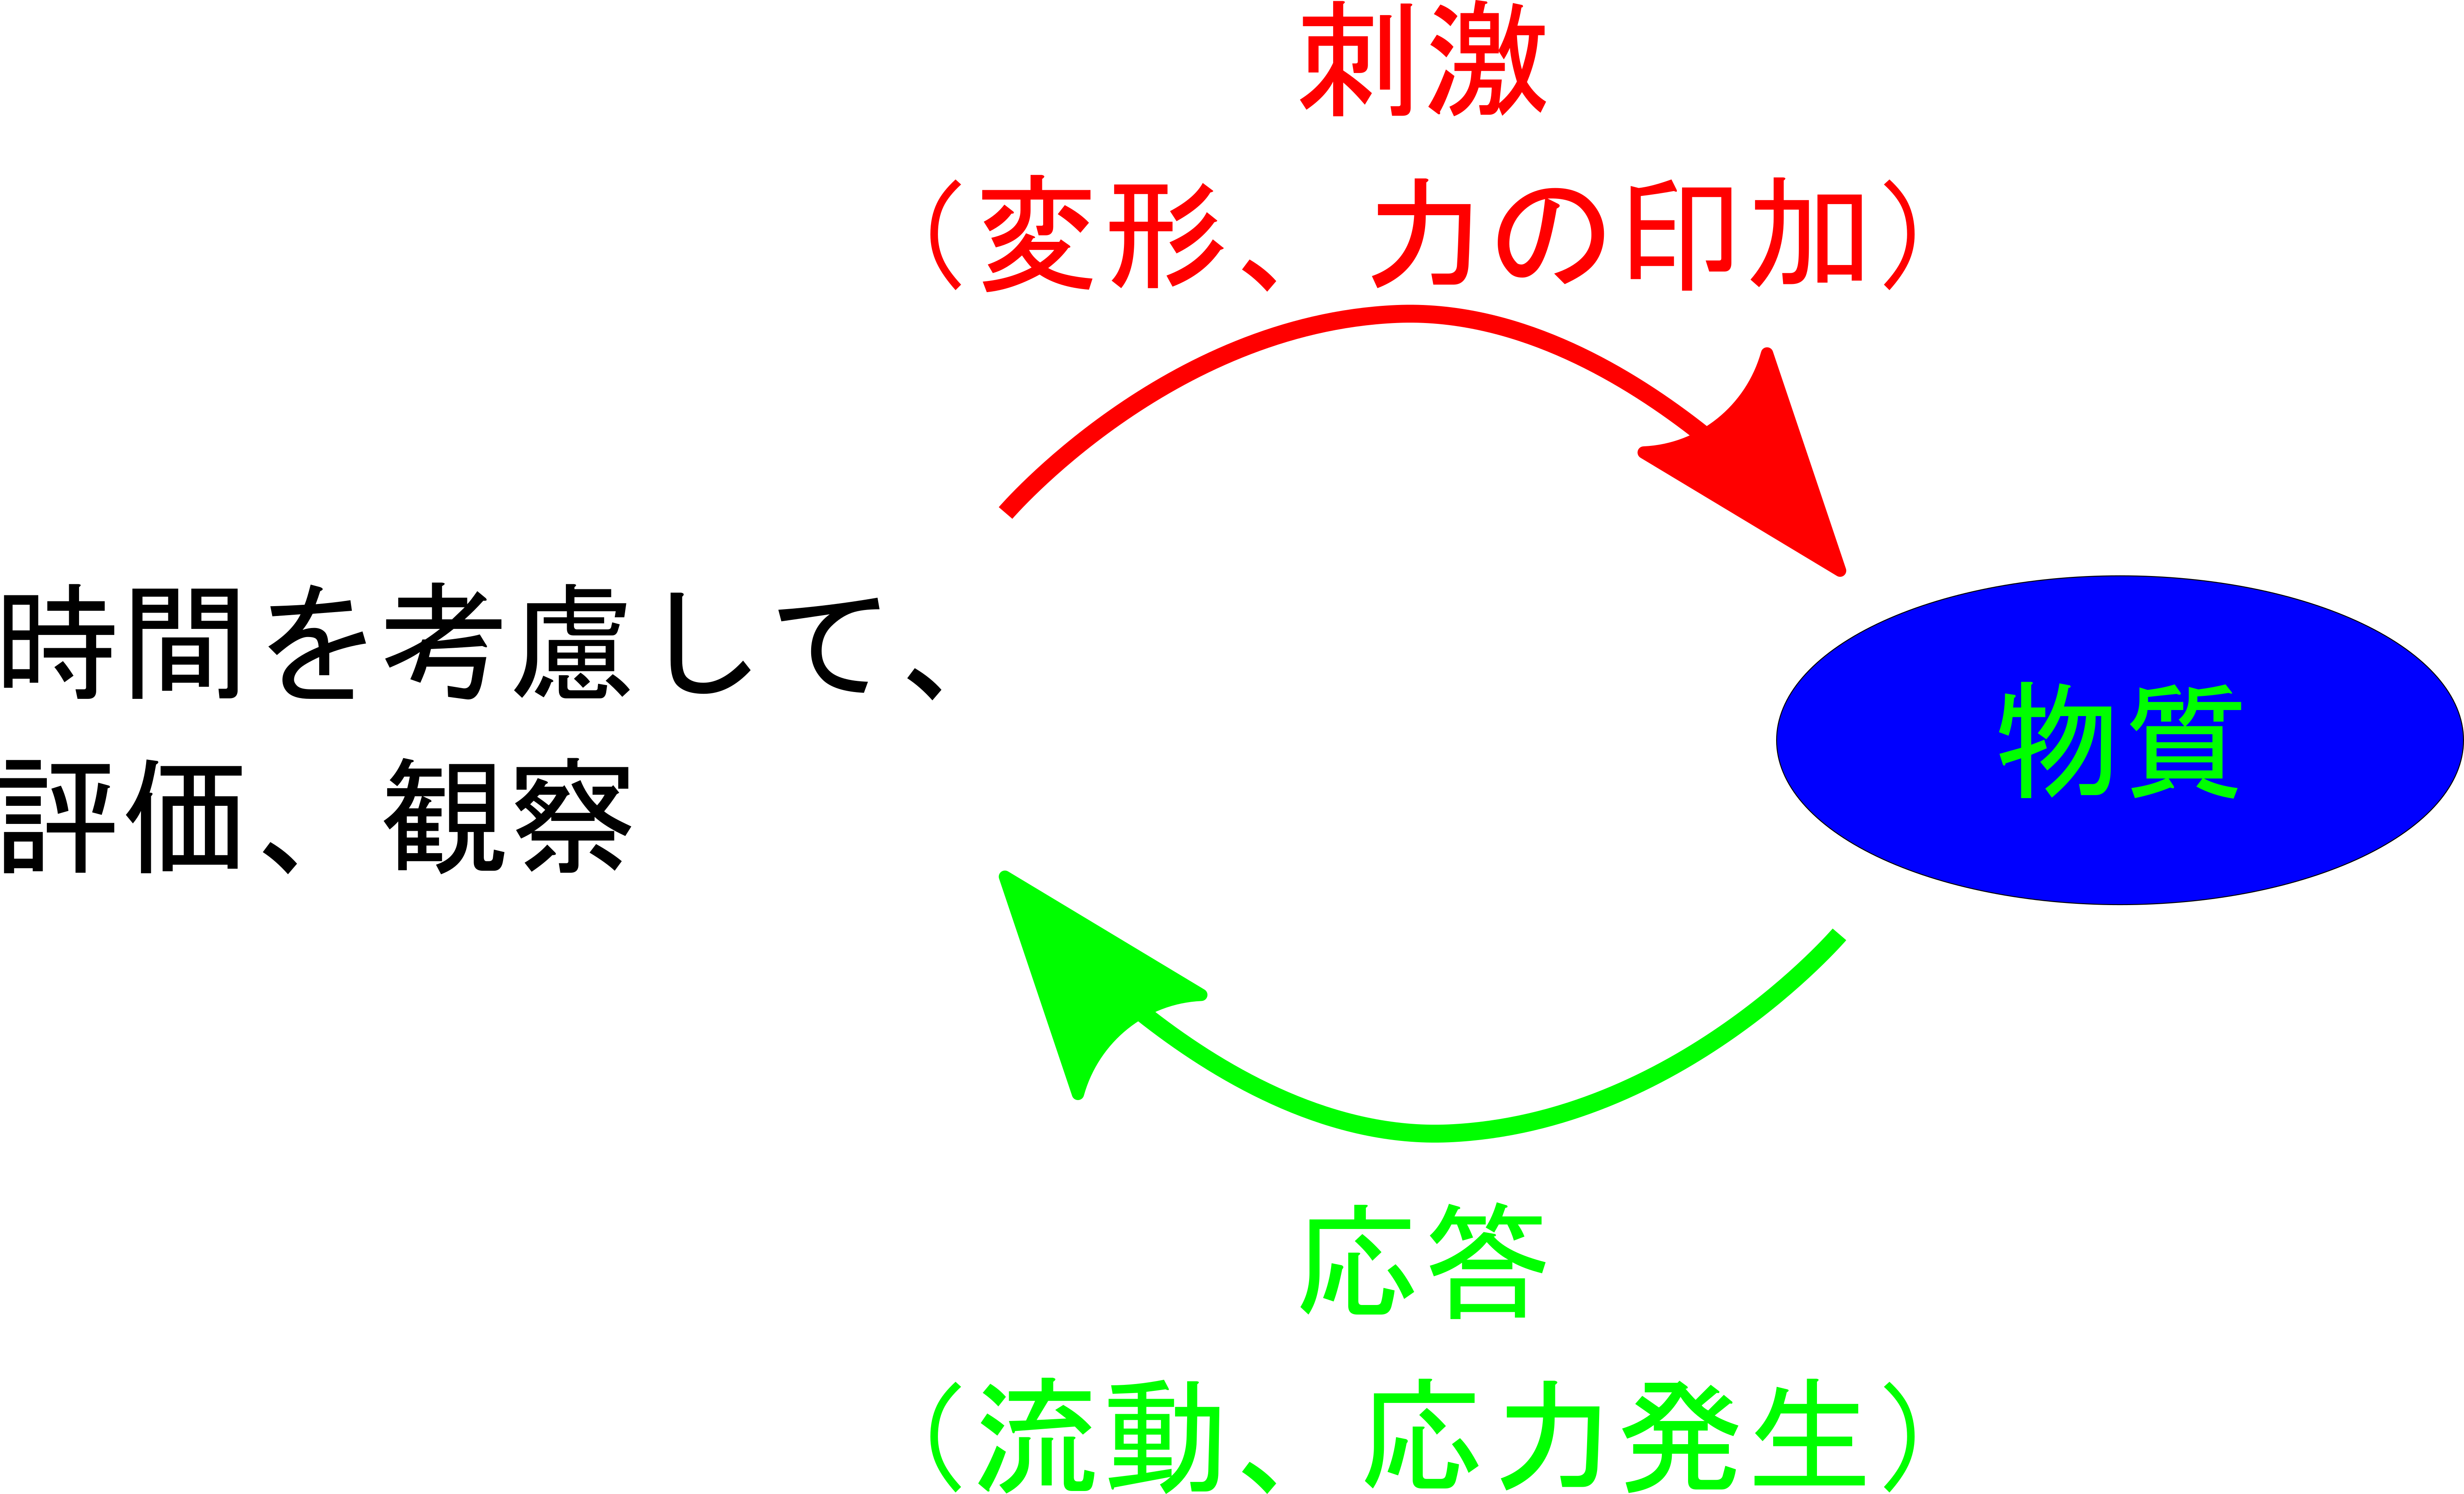
\includegraphics[width=.9\textwidth]{Rheo_method.png}
        \caption{レオロジーのやりかた}
        \label{yarikata}
    \end{center}
\end{figure}

レオロジーは、弾性固体\index{こたい@固体}とか粘性流体のような「理想的な物体」に限ること無く、我々が日々に遭遇する「一般にそこらに存在する物質や材料」を対象に含んでいます。
言い換えれば、対象を問わず、その変形と流動\index{りゅうどう@流動}に関する事柄をすべて取り扱うということになり、物理学、化学、生物学、地学、医学、薬学、農学、食品学、家政学、時には心理学までをも含む多くの学問分野に横断的に関係する極めて学際的な学問となっています。

レオロジーは、そもそも科学の一分野として提唱されたわけですが、変形や流動\index{りゅうどう@流動}というキーワードで物質や材料の特性を評価できることになりますから、実学として工学的にも大きな意味を持って来ています。
これが、広くレオロジーが用いられるようになった大きな要因となります。

レオロジーを測定する具体的な方法は、物質に外的な刺激を与えて、その応答としての変形や流動\index{りゅうどう@流動}を測ることになります。
一般に、その刺激とは物質に力\index{ちから@力}や変形を与えることであり、応答としては時間という因子を意識しながら物質の流動や返してくる力\footnote{
	このあとに詳細を学びますが、このときの返してくる力は「応力\index{おうりょく@応力}」という物質内部での内力と呼ばれるものとなります。
}を測定することになります。
そして、このような測定を通して、物質の持つ各種の特性を比較することができるようになるわけです。

この考え方を簡単に書き直すと、図 \ref{yarikata} に示したようになります。

\section{会社の仕事とレオロジー}

ここでは、レオロジーの関わる分野が多様であることを確認し、その多様性を会社の仕事に生かしていくということについて考えてみましょう。

\subsection{レオロジーの関わる分野}

前述したように、1929年にアメリカにおいて、Bingham を中心としてレオロジー学会 The Society of Rheology (SOR) が設立されました。
日本では、それから約二十年後の 1951 年に第1回レオロジー討論会が開催されています。
その後、多様な分野へとその適応される範囲は広がってきています。

例えば、2019 年に開催された第 67 回レオロジー討論会に協賛した学会を見てみましょう。
\begin{screen}
	日本材料学会、プラスチック成形加工学会、高分子学会、日本化学会、日本物理学会、繊維学会、応用物理学会、化学工学会、
	強化プラスチック協会、日本ゴム協会、日本接着学会、日本セラミックス協会、日本木材学会、セルロース学会、日本機械学会、
	日本雪氷学会、日本混相流学会、日本流体力学会、可視化情報学会、日本食品科学工学会、日本家政学会、日本調理科学会、
	日本食品工学会、日本繊維機械学会
\end{screen}

非常に多様な学会が協賛しており、レオロジーという学問が学際的な特徴を有していることがわかります。

さらに、それぞれの学会が関連している分野を考えると、学術的な分類だけではなくて材料の種類や応用の範囲にしても、以下のように非常に幅広い分野に渡っていることが理解できます。
	\begin{itemize}
	\item
	  学術分野:化学、物理、生物、化学工学、応用物理、流体力学、地球物理学
	\item
	  高分子化学(科学):プラスチック、繊維、ゴム、強化プラスチック
	\item
	  材料:金属、セラミックス、木材
	\item
	  応用:機械、接着、塗料、食品化学、調理科学、家政学、成型加工
	\end{itemize}
	
したがって、レオロジーとは、高度に学際的な科学であると同時に、それぞれの要素技術が大きく異る多岐にわたる対象を、多様な切り口で議論していくことが出来るアプローチとも捉えられます。

\begin{figure}[htb]
	\begin{center}
		\includegraphics[width=.9\textwidth]{Katsuyou.png}
		\caption{レオロジーの活用}
		\label{katsuyou}
	\end{center}
\end{figure}

\subsection{会社の仕事とレオロジー}

次に、会社の仕事とレオロジーの関係について考えてみましょう。
この講座に参加されているみなさんの大多数は、会社に勤務されていると思います。
ここで、会社の社会的な意味について確認しておきましょう。

一般に、会社は営利団体であり、利益を生み出すことでその存在を継続させ、社会的な意義を果たしていくことになります。
そして、製造に関連する会社であれば、商品(製品)を作り出し、製造、販売することで、その利益を生じているわけです。

商品の開発の流れを簡単に言えば、原料から材料、そして商品へと価値を付与できるようにつなげていく過程と考えることができます。
そして、それぞれのステップで評価・解析に基づく、設計を行っていくわけです。
その設計の過程において商品に必要となる特性を評価する際に、レオロジーを活用することが多いわけです。
模式図とすれば、図 \ref{katsuyou} に示したようなイメージとなります。

\subsection{レオロジーと商品}

以前に図示(図 \ref{yarikata})したように、レオロジーとは物質に刺激を与えてその応答を評価観察することで、その特性を評価できるのでした。

では、商品化におけるレオロジー利用の、具体的な例を見てみましょう。
以下に示したように、人間の心地良さの定量化や、原料、材料の機能設計にレオロジーが活用されている事例が多くあります。
\large
	\begin{itembox}[l]{レオロジーが活用されている例}
		\begin{itemize}
			\item
			人間の心地良さの定量化にレオロジー的感覚で評価
			\begin{itemize}
				\item 食品工学における「舌触り」や「のど越し」のような食感の定量化。
				\item 肌触りの良い下着やノビの良い化粧品のような触感の定量化
			\end{itemize}
			\item
			原料、材料の機能設計にレオロジーを利用
			\begin{itemize}
			\item
				ショックのない運動靴やよく飛ばせるゴルフクラブのような力学特性の評価
			\item
				塗り易くて液だれしない塗料のような流動特性の評価
			\end{itemize}
		\end{itemize}
	\end{itembox}
\normalsize
したがって、少なくとも定性的に物事を評価するためには、レオロジーが非常に有効な方法であることが理解できるでしょう。

\section{人の感覚とレオロジー}
\label{sec:1_kankaku}

前節で、人間の心地良さのような感覚を評価するためにレオロジーが使えるという事例を示しました。
このことについて、もう少し詳しく考えてみましょう。

\subsection{人はみなレオロジスト}

\subsubsection{オノマトペとレオロジー}

オノマトペ\index{おのまとぺ@オノマトペ}とは、状態や感情を言葉に表したものであり、この語彙が多彩で豊富であることが日本語の大きな特徴の一つとなっています。
織物などの手触りのような質感を意味する言葉として、テクスチャという言葉もあります。
手触りだけでなく食品分野で食感を表現するためにも、テクスチャを表すオノマトペが多用されています。

レオロジーに、単純につながるような物性を表す言葉としては、「サラサラは低粘度、ドロドロは高粘度」や「ふにゃふにゃは低弾性、カチカチは高弾性」のようなものもありますし、これが、フワッフワとかモッチモチになると、一層感覚的な表現になってきます。
このような感覚は、別に若者言葉として特別なのではなくて、日本人には共通認識として通じる感覚になっています。
\begin{figure}[htb]
	\begin{center}
		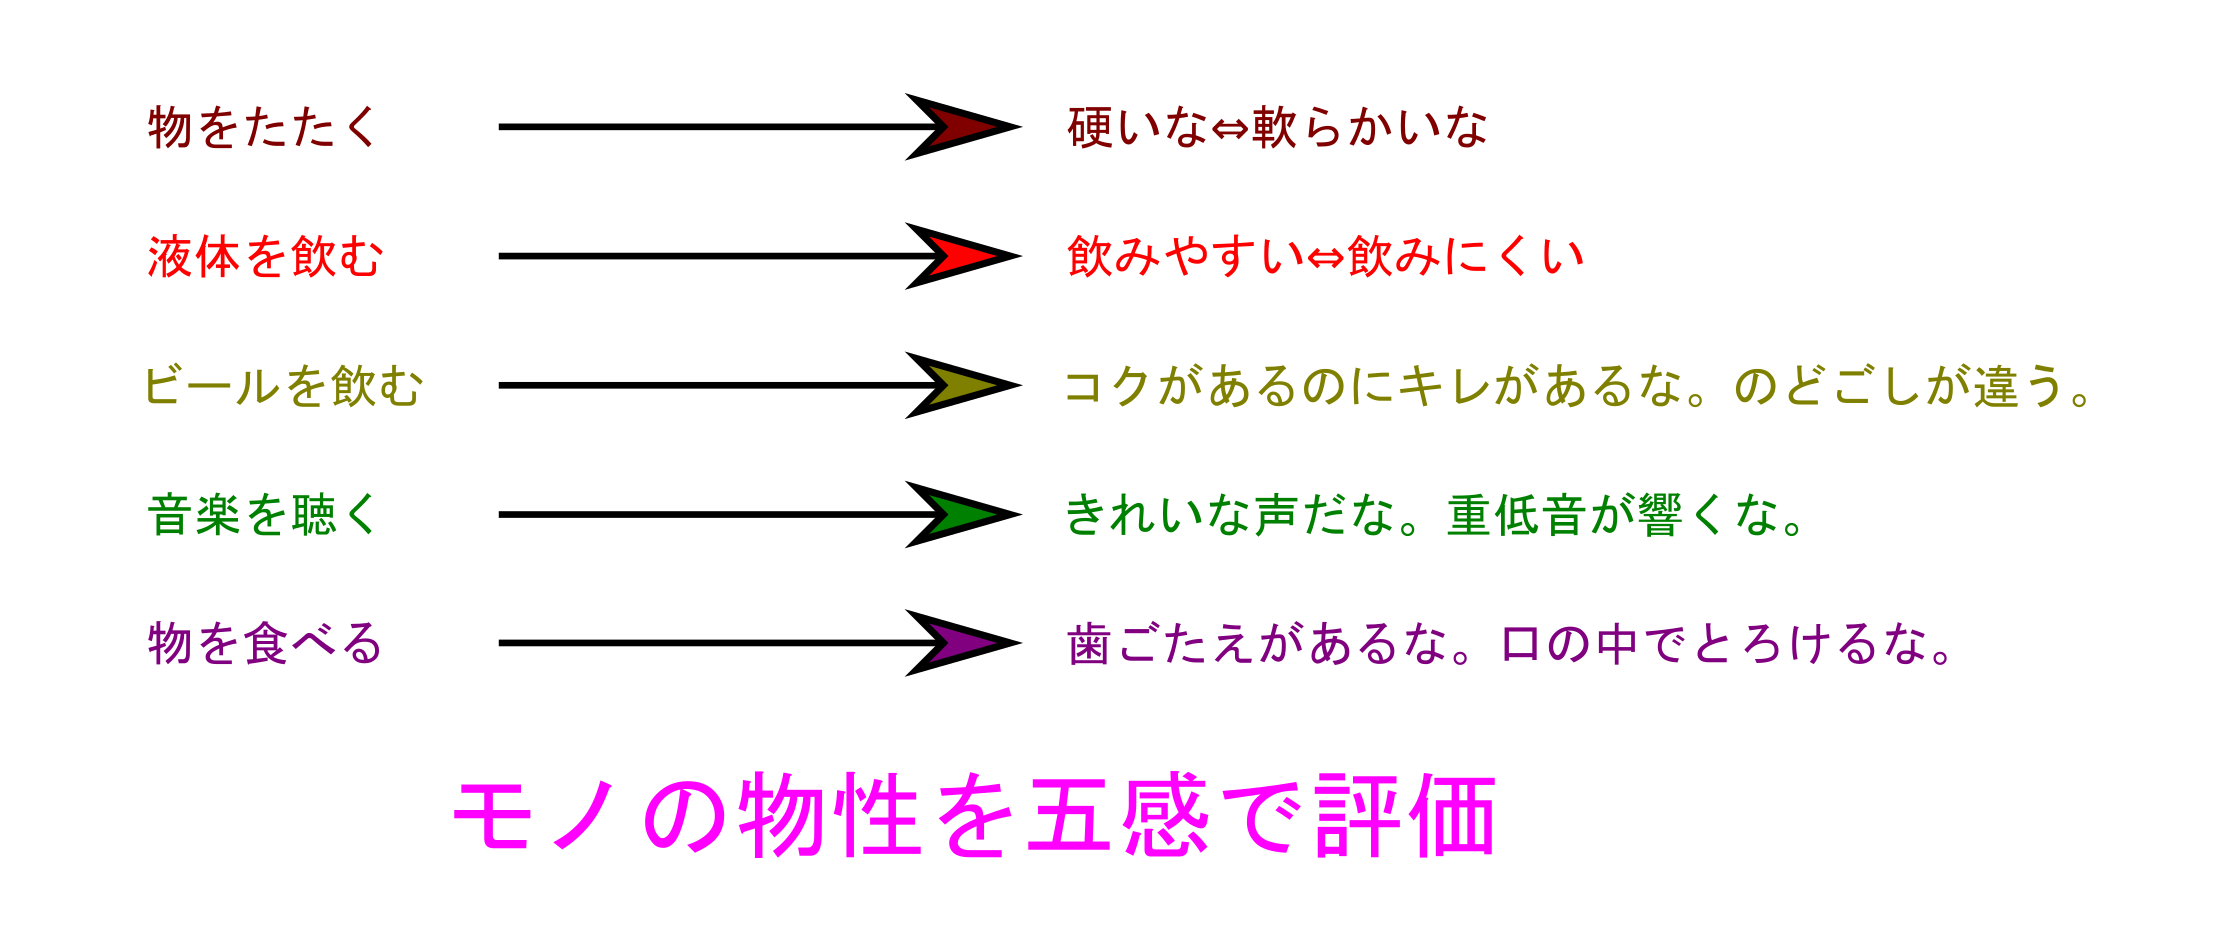
\includegraphics[width=.9\textwidth]{gokan.png}
		\caption{人間の五感とレオロジー}
		\label{gokan}
	\end{center}
\end{figure}

そして、このような言葉として物性やモノの有り様を表すことは、科学としてのレオロジーだけではなく、日常的に行われている評価なのです。

\subsubsection{人間の五感とレオロジー}

我々の生活の場において、なにかものを評価するときに、それを叩いてその音で判断することがあります。
具体的には、以下のような場面です。

\begin{itemize}
	\item 陶磁器の品質を見分ける
	\begin{itemize}
		\item 指先ではじいてその音を聞く
		\item 焼き上がり具合に応じて振動状態が変化し、陶器と磁器の見分けがつく。
	\end{itemize}
	\item スイカの熟し具合
	\begin{itemize}
		\item 熟れ過ぎたスイカは音が低くなる。
		\item 実の部分に微小な気泡が生じている。
	\end{itemize}
	\item 医者が打診によって診断
	\begin{itemize}
		\item お医者さんが指で胸やお腹を叩く。
		\item 音の響きで、内臓の腫れやうっ血を判断できる。
	\end{itemize}
\end{itemize}

こんな具合に、人は物質の状態を音で判断することができているわけです。

また、手触りでものの状態を判断することもやっています。
これらの行為は、ものを叩いたり触ったりして刺激を与えて、その応答を音で聞いたり手触りで感じたりしているわけですから、レオロジー評価を行っていると言うことにほかなりません。
すなわち、人間は五感を使ってレオロジーを行うレオロジストということになります。

\subsection{人間の判断基準は?}

しかしながら、オノマトペのような言葉としての表現はあくまでも感覚としての相対的な比較であり、感覚としての違いを何でどのように表すかが難しいわけです。

具体的な数値化のお話は後で行いますが、ここでは、人間の感覚の特徴について、もう少し考えてみましょう。

\subsubsection{ウェーバー比\index{うぇーばーひ@ウェーバー比}}

様々な刺激に対する人間の感覚的な評価について、ドイツの生理学者である E. Weber は、「人間の変化を感じ取る感覚量は、受ける刺激の差ではなく何倍になったかという比に依存する」という関係を見出しました。
\begin{align*}
	\text{ウェーバー比} = \dfrac{\Delta R}{R}= \dfrac{\text{増加量}}{\text{初期値}}
\end{align*}

\begin{figure}[htb]
	\begin{center}
		\begin{minipage}{0.45\textwidth}
			\large
			\begin{itembox}[l]{ウェーバー比}
				\begin{itemize}
					\item 人間の感覚量は、
					\item 受ける刺激の差ではなく、
					\item 何倍になったかという比
				\end{itemize}
			\end{itembox}
		\end{minipage}
		\begin{minipage}{0.45\textwidth}
			\large
			\begin{align*}
				\text{ウェーバー比} &= \dfrac{\Delta R}{R} \\
				&= \dfrac{\text{増加量}}{\text{初期値}}
			\end{align*}
		\end{minipage}
		\caption{ウェーバー比}
		\label{fig:weber}
	\end{center}
\end{figure}

この関係を数式で表すと、はじめに加えられる基準となる刺激量の強度を $R$ としたとき、人間が違いに気づくことができる閾値 $\Delta R$ との間に以下のような式が成立し、そのウェーバー比は事柄ごとに決まるということになります。

これを具体的に書くと、ある人が、10 の刺激が 20 になったときに「増加した」と気づくとしましょう。
このときの増加量は、10になりますから、ウェーバー比は 1 です。
その人は、20 の刺激が同じ増加量で 30 になってもその増加には気づかず、気づかせるためには 40 にする必要があるということになります。
言い換えると、「もともと強い刺激を基準とした場合、その違いを見分けることは難しい。$\Leftrightarrow$ 強い刺激には鈍感」ということになります。

当然、人の感覚は異なりますから、ウェーバー比の値は個々に異なりますが、大枠の傾向としてはこの様になっているわけです。

\subsubsection{フェヒナーの法則}

ヴェーバーの弟子である G. Fechner は、ヴェーバーの法則の式を微分方程式とみなして積分することにより、以下の対数法則を導き出しています。

すなわち、刺激量の強度 $R$ が変化する時、これに対応して人が感じる感覚量 $E$ は、以下のようになります。
\begin{align*}
	E = C \log R
\end{align*}
ここで $C$ は定数です。

この数式の示すことは、心理的な感覚量 $E$ は、刺激の強度の値 $R$ ではなく、その対数\index{たいすう@対数} $\log R $ に比例して知覚されるということになります。
具体的に言えば、100 の刺激が倍に増加して 200 になるときの感覚量と、200 の刺激が倍に増加して 400 になるときの感覚量の変化は等しいわけです。

\subsubsection{ウェーバー・フェヒナーの法則\index{うぇーばー・ふぇひなーのほうそく@ウェーバー・フェヒナーの法則}}

二人の師弟によって示された上記の関係を合わせてまとめると、
\large
	\begin{itembox}[l]{ウェーバー・フェヒナーの法則}
		\begin{itemize}
			\item 刺激量の差だけではわかりにくい
			\begin{itemize}
				\item 相対変化は見やすいが、絶対的な差はわかりにくい。
			\end{itemize}
			\item 基準値によって閾値が変わる
			\begin{itemize}
				\item 元々強い刺激の変化には鈍感
				\item 基準値をそろえたほうがわかりやすい。
			\end{itemize}
			\item 差ではなく比で比較する
			\begin{itemize}
				\item 桁数の違いで感じるということが大事。
			\end{itemize}
		\end{itemize}
	\end{itembox}
\normalsize
というようなことになります
\footnote{
	ここで議論したような人間の感覚に関わるような分野は、心理レオロジー(サイコレオロジー)と呼ばれており、定性的な感覚量を定量化するためには重要な考え方になっています。
}
。

このように考えると、レオロジー評価を料理に例えられる場合の以下のような表現も理解できてきます。
\begin{itemize}
	\item レオロジーで何がわかるのか?
	\begin{itemize}
		\item 隠し味の調味料がわかるわけではない!
		\item 調味料を加えた時に、味がどう変化したのかがわかる。
	\end{itemize}
	\item 比較試料を用いて、相対値評価をする
	\begin{itemize}
		\item 絶対値評価はできない。
		\item 対数的な応答と考えれば、理解しやすい。
	\end{itemize}
\end{itemize}

\section{レオロジーを理解するために}
\subsection{レオロジーの難しい点}

前述のように、レオロジーという考え方自体は非常に単純で分かりやすいものなんですが、
実際に比較しようとするととたんに面倒くさくなってくるものでもあります。

\subsubsection{似たものを比べると?}

例えば、身近にある水と蜂蜜を比べてみましょう。
\begin{itemize}
	\item 水
	\begin{itemize}
		\item 箸で簡単にかき混ぜることができる。
		\item たやすくコップに注ぎ込むことができる。
	\end{itemize}
	\item 蜂蜜
	\begin{itemize}
		\item 容易にかき回すことができない。
		\item 入れ物を傾けても、流れにくい。
	\end{itemize}
\end{itemize}

触ってみたときの手応えとして比べるのであれば、これらの二つがずいぶん違うことは簡単にわかります。
しかしながら、その違いはあくまでも感覚としての相対的な比較であり、この違いを何で表すかが難しいわけです。

粘っこい者同士となると一層困難になります。
例えば、ハチミツとマヨネーズとを比べることを考えてみましょう。 
これらを比較するためには、何らかの客観的な判断基準が必要となってくることになります。

\subsubsection{言葉の使い方が曖昧}

もう一つの面倒くさいこととして、レオロジーでは多様な言葉が用いられる場合が多いことが挙げられます。
これは、\ref{sec:1_kankaku} 節 (\pageref{sec:1_kankaku} ページ) で後述するように、
レオロジーが人間の直感的な評価を行いやすいためだと考えることができます。
その結果として、抽象的な言葉や指示代名詞による、あまりにもイメージに偏った議論に陥りがちになるのです
\footnote{まあ、流石に以下のようなことを本当に言う人は少ないのですが、それに近いことを口走っていることはよく見かけます。
	
「この時はこう、あの時はああ。」$\Leftarrow$ それなら。今はどの時?}。

例えば、以下に示したように、言葉の定義や使い方が不明確だとわかりにくくなります。
% \begin{shadebox}
	
	\begin{itemize}
		\item わかり易そうで、油断するとよくわからない表現(逃げ言葉?)\\
		たとえば、以下に示したような言葉は、レオロジーの説明によく出てきていますが、
		具体的に理解しようとするとその意味がとたんにわからなくなりませんか?
		\begin{itemize}
			\item 「応力集中が粘弾性により緩和します。」
			\item 「チクソ性の高い液体は液だれしにくい。」
			\item 「非Newton 流体の特徴的な流動を設計しなければいけない。」
		\end{itemize}
		\item 数式の羅列で数学的なお話\\
		確かに、数式を使いこなせれば言葉の定義の不明確さは解消できるのですが、数式が突然天下りで出てきても、
		内容がイメージできるわけでもありません。なお、以下の表式は見た目がややこしそうというだけの例です。
		\begin{itemize}
			\item 例えば、一般化マックスウェルモデルの動的貯蔵弾性率を表す数式\\
		\end{itemize}
	\end{itemize}
	\vspace{-7mm}
	\begin{align*}
		\displaystyle G'(\omega) = \int_{-\infty}^{\infty} \mathcal{H}(\ln \tau)\dfrac{\omega^2 \tau^2}{1 + \omega^2 \tau^2} \mathrm{d}(\ln \tau)
	\end{align*}
% \end{shadebox}

さらに、レオロジーの対象は非常に幅広いものであることも、混乱しやすいもう一つの原因となります。
以下に例を示したように、食感や手触りから、材料の機能性の設計に至るまで、非常に幅広い分野でレオロジーの言葉は使われています。
これらの言葉も、使っている人に応じて微妙に言葉に込めた意味合いが異なっていますので、混乱しやすいものとなります。
% \begin{shadebox}
	\begin{itemize}
		\item 人間の心地よさをレオロジー的感覚で評価
		\begin{itemize}
			\item 「タピオカ」の喉越しのツルンとした感覚
			\item 肌触りのよい下着
		\end{itemize}
		\item 機能設計にレオロジーを利用
		\begin{itemize}
			\item ショックのない運動靴
			\item 塗り易くて液だれしない塗料
		\end{itemize}
	\end{itemize}
% \end{shadebox}

\subsubsection{よくある状態}

我々の身の回りで、レオロジー関連で実際によくある状態として、以下のようなものがあります。
たとえば、「頭で考えずに手を動かして、とにかく測れ」と言われたり、「まずよく調べてから測定しよう」と言われたりして、
どうすればいいのか判らなくなったりします。
そこで、自身が素人であることを自覚して周りのマネをしようとしても、近くに先輩がいなかったり、
そもそも新しい問題については誰も先輩になれなかったりもするわけです。
\large
	\begin{itembox}[l]{よくある状態}
		\begin{itemize}
			\item ありがちな両極端
			\begin{itemize}
				\item 脳みそ筋肉状態
				\begin{itemize}
					\item とにかく測れ
				\end{itemize}
				\item 頭でっかち
				\begin{itemize}
					\item 理屈ばかりで手が動かない
				\end{itemize}
			\end{itemize}
			\item 誰もが、最初は素人 $\Leftrightarrow$ うまくやっている人の物まねが手っ取り早い
			\begin{itemize}
				\item でも、近くにいい先輩がいないときは?
				\item 新しい問題へのアプローチは?
			\end{itemize}
		\end{itemize}
	\end{itembox}
\normalsize

\subsection{理解へのアプローチ}
こんなときに、おすすめしたいのが、
\begin{center}
	\Huge{\bf「急がば回れ」}
\end{center}
という、キーワードになります。

すなわち、慌てて結果を出そうとするのではなく、心を落ち着けてやるべきことを明確化してイメージすることから始めてみることをお勧めします。

レオロジーというややこしいものでも、イメージとして全体像をザックリと捕まえることができれば、理解は一気に容易になります。

\subsubsection{見える化のすすめ}

イメージとして捉えるためには、自分の捉えるべき問題を自分の中に落とし込むことが大事です。
そのためには、モチベーションを高くすることが重要だと思います。
\large
\begin{itembox}[l]{お勧めの考え方}
	\begin{itemize}
		\item 「何のためにやりたいのか?」を明確に。
		\begin{itemize}
			\item 目的がわからないと、ゴールが見えない。
			\item 仕事であれば、上司とよく相談。
			\item 自己啓発であれば、自分の本心をよく見極める。
		\end{itemize}
		\item 「何をやりたいのか?」を常に意識しながら、
		\begin{itemize}
			\item 因果関係をはっきりと
			\begin{itemize}
				\item 因 $\Leftarrow$ 原因
				\item 果 $\Leftarrow$ 結果
			\end{itemize}
			\item 図として捉える
			\begin{itemize}
				\item 複雑な実事象をできるだけ単純化
				\item 一目で理解できるように  
			\end{itemize}
		\end{itemize}
	\end{itemize}
\end{itembox}
\normalsize



つまり、たとえ会社の仕事として命令されたような事項であっても、「何のためにやりたいのか」という目的と
「何をやりたいのか」という目標をきちんと設定することが最も大事になるのです。
他人事ではなく自分の問題として捉えることで、やる気が全く変わってくるものです。

そして、因果関係をはっきりとさせながら、その関係を図として単純化したイメージが持てるようになれば、
目標とそこに到達するための手段もクリアーに落とし込むことが出来ると感じています。

\subsubsection{色々なモデル化\index{もでるか@モデル化}}
それでは、レオロジーという道具を理解して、私達は何をやりたいのでしょうか?

この答えは、みなさんがそれぞれ異なっているでしょう。

参考までに著者の場合を書けば、私は「様々な条件のもとで幅広い検討対象に対してでも当てはめることの出来るような、
汎用的なモデル」が欲しいと考えています。
このモデルは、多様な実験事実を「尤もらしく」説明できるものであってほしいと考えています。
このような考え方ができるようになることで、表面的には異なる問題に見えるようなものの本質を捕まえることが出来、
普遍的な問題として捕まえることが出来ると信じています。
特に、レオロジーのようにとらえどころのないややこしい問題に対しては、適度に単純化したモデルが有効だと感じてきました。

これからの具体的な説明の中において、この「モデル化」という考え方についても、実際の例を上げて説明していきます。

\large
\begin{itembox}[l]{モデル化のすすめ}
	\begin{itemize}
		\item 適度な深さで尤もらしく
			\begin{itemize}
				\item 簡単すぎるものは例外が多い。
				\item 複雑化しすぎても過適応
				\begin{itemize}
					\item n個のデータを、n次の関数でフィット
					\item 個々の現象にだけ適応可能
					\item モデル化する意味がない
				\end{itemize}
			\end{itemize}
		\item 欲しいもの
		  \begin{itemize}
			\item 汎用的に使えるモデル
			\item 尤もらしく、実験事実を説明できるもの
		  \end{itemize}
		\end{itemize}
\end{itembox}
\normalsize

\section{この章のまとめ}
この章では、レオロジーという「考え方」についての説明を行い、会社の仕事にどのように役立つかを考え、
「おすすめの理解へのアプローチ」について紹介しました。
\begin{boxnote}
	\large
	\begin{itemize}
		\item 「レオロジー」という言葉の歴史的背景を振り返り、その流れを確認
		\item レオロジーが関わる分野が広範囲に渡り、会社での商品開発に有用
		\item 人間の直感とレオロジーの親和性が高いこと
		\item 「おすすめの理解へのアプローチ」について紹介
	\end{itemize}
\end{boxnote}

\newpage

\begin{longartdeco}
	\begin{center}
	\emph{コラム:緩和とリラックス}	
	\end{center}

	レオロジーという学問は、その成り立ちをベースにすれば、「流れるものの流れ方を考える学問」と捉えることができます。
	
	単純な応答を示す水のように、明らかに液体的な性質が主となってい場合には、あまり面倒なことを考える必要はありません。
	この場合は、変形速度と応力の関係を表す比例定数である粘度を決定すれば、流れ方の特徴を理解したことになります。
	このような流体は、初期の研究を行った Newton に因んでニュートン流体と分類されています。
	
	でも、世の中の大多数の物質はそれほど単純ではありません。
	一般に、固体的な性質と液体的な性質を兼ね備えた「粘弾性」という性質を持っている物質が多数派となっています。
	
	レオロジーでは、流れるということを「変形という刺激を与えた結果として生じる応答」と考えます。
	このような考え方に立てば、与えた刺激(変形)が消滅していく過程こそが「刺激が緩和していく」ということに対応します。
	したがって、粘弾性を示す物質においては、その「緩和現象」が重要になってくることになります。
	
	最後にゆったりとしたお話で締めましょう。
	緩和という言葉は、英語ではリラックスとなります。
	この語源はラテン語で、「緩んた状態(laxare)へ戻す(re)」ということを意味しているようです。
	昼間の仕事時間に、職場で拘束されて固体的にきちんと振る舞っていたサラリーマンが、
	自宅に帰ってソファーの上でだらけて液体的にリラックスしていく過程も緩和なんでしょうね。

\end{longartdeco}

\end{document}